\documentclass[a4paper,12pt,twoside]{memoir}

% Castellano
\usepackage[spanish,es-tabla]{babel}
\selectlanguage{spanish}
\usepackage[utf8]{inputenc}
\usepackage[T1]{fontenc}
\usepackage{lmodern} % scalable font
\usepackage{microtype}
\usepackage{placeins}
\usepackage{listings}
\usepackage{dirtree}
\usepackage{adjustbox}


\RequirePackage{booktabs}
\RequirePackage[table]{xcolor}
\RequirePackage{xtab}
\RequirePackage{multirow}

\lstset{
  basicstyle=\ttfamily,
  columns=fullflexible,
  frame=single,
  breaklines=true,
  postbreak=\mbox{\textcolor{red}{$\hookrightarrow$}\space},
}

% Links
\PassOptionsToPackage{hyphens}{url}\usepackage[colorlinks]{hyperref}
\hypersetup{
	allcolors = {red}
}

% Ecuaciones
\usepackage{amsmath}

% Rutas de fichero / paquete
\newcommand{\ruta}[1]{{\sffamily #1}}

% Párrafos
\nonzeroparskip

% Huérfanas y viudas
\widowpenalty100000
\clubpenalty100000

% Evitar solapes en el header
\nouppercaseheads

% Imagenes
\usepackage{graphicx}
\newcommand{\imagen}[2]{
	\begin{figure}[!h]
		\centering
		\includegraphics[width=0.9\textwidth]{#1}
		\caption{#2}\label{fig:#1}
	\end{figure}
	\FloatBarrier
}

\usepackage{graphicx}
\newcommand{\imagenSized}[3]{
	\begin{figure}[!h]
		\centering
		\includegraphics[width=#3\textwidth]{#1}
		\caption{#2}\label{fig:#1}
	\end{figure}
	\FloatBarrier
}

\newcommand{\imagenflotante}[2]{
	\begin{figure}%[!h]
		\centering
		\includegraphics[width=0.9\textwidth]{#1}
		\caption{#2}\label{fig:#1}
	\end{figure}
}



% El comando \figura nos permite insertar figuras comodamente, y utilizando
% siempre el mismo formato. Los parametros son:
% 1 -> Porcentaje del ancho de página que ocupará la figura (de 0 a 1)
% 2 --> Fichero de la imagen
% 3 --> Texto a pie de imagen
% 4 --> Etiqueta (label) para referencias
% 5 --> Opciones que queramos pasarle al \includegraphics
% 6 --> Opciones de posicionamiento a pasarle a \begin{figure}
\newcommand{\figuraConPosicion}[6]{%
  \setlength{\anchoFloat}{#1\textwidth}%
  \addtolength{\anchoFloat}{-4\fboxsep}%
  \setlength{\anchoFigura}{\anchoFloat}%
  \begin{figure}[#6]
    \begin{center}%
      \Ovalbox{%
        \begin{minipage}{\anchoFloat}%
          \begin{center}%
            \includegraphics[width=\anchoFigura,#5]{#2}%
            \caption{#3}%
            \label{#4}%
          \end{center}%
        \end{minipage}
      }%
    \end{center}%
  \end{figure}%
}

%
% Comando para incluir imágenes en formato apaisado (sin marco).
\newcommand{\figuraApaisadaSinMarco}[5]{%
  \begin{figure}%
    \begin{center}%
    \includegraphics[angle=90,height=#1\textheight,#5]{#2}%
    \caption{#3}%
    \label{#4}%
    \end{center}%
  \end{figure}%
}
% Para las tablas
\newcommand{\otoprule}{\midrule [\heavyrulewidth]}
%
% Nuevo comando para tablas pequeñas (menos de una página).
\newcommand{\tablaSmall}[5]{%
 \begin{table}
  \begin{center}
   \rowcolors {2}{gray!35}{}
   \begin{tabular}{#2}
    \toprule
    #4
    \otoprule
    #5
    \bottomrule
   \end{tabular}
   \caption{#1}
   \label{tabla:#3}
  \end{center}
 \end{table}
}

% Nuevo comando para tablas pequeñas (menos de una página).
\newcommand{\tablaSmallFija}[5]{%
 \begin{table}[H]
  \begin{center}
   \rowcolors {2}{gray!35}{}
   \begin{tabular}{#2}
    \toprule
    #4
    \otoprule
    #5
    \bottomrule
   \end{tabular}
   \caption{#1}
   \label{tabla:#3}
  \end{center}
 \end{table}
}

%
%Para el float H de tablaSmallSinColores
\usepackage{float}

%
% Nuevo comando para tablas pequeñas (menos de una página).
\newcommand{\tablaSmallSinColores}[5]{%
 \begin{table}[H]
  \begin{center}
   \begin{tabular}{#2}
    \toprule
    #4
    \otoprule
    #5
    \bottomrule
   \end{tabular}
   \caption{#1}
   \label{tabla:#3}
  \end{center}
 \end{table}
}

\newcommand{\tablaApaisadaSmall}[5]{%
\begin{landscape}
  \begin{table}
   \begin{center}
    \rowcolors {2}{gray!35}{}
    \begin{tabular}{#2}
     \toprule
     #4
     \otoprule
     #5
     \bottomrule
    \end{tabular}
    \caption{#1}
    \label{tabla:#3}
   \end{center}
  \end{table}
\end{landscape}
}

%
% Nuevo comando para tablas grandes con cabecera y filas alternas coloreadas en gris.
\newcommand{\tabla}[6]{%
  \begin{center}
    \tablefirsthead{
      \toprule
      #5
      \otoprule
    }
    \tablehead{
      \multicolumn{#3}{l}{\small\sl continúa desde la página anterior}\\
      \toprule
      #5
      \otoprule
    }
    \tabletail{
      \hline
      \multicolumn{#3}{r}{\small\sl continúa en la página siguiente}\\
    }
    \tablelasttail{
      \hline
    }
    \bottomcaption{#1}
    \rowcolors {2}{gray!35}{}
    \begin{xtabular}{#2}
      #6
      \bottomrule
    \end{xtabular}
    \label{tabla:#4}
  \end{center}
}

%
% Nuevo comando para tablas grandes con cabecera.
\newcommand{\tablaSinColores}[6]{%
  \begin{center}
    \tablefirsthead{
      \toprule
      #5
      \otoprule
    }
    \tablehead{
      \multicolumn{#3}{l}{\small\sl continúa desde la página anterior}\\
      \toprule
      #5
      \otoprule
    }
    \tabletail{
      \hline
      \multicolumn{#3}{r}{\small\sl continúa en la página siguiente}\\
    }
    \tablelasttail{
      \hline
    }
    \bottomcaption{#1}
    \begin{xtabular}{#2}
      #6
      \bottomrule
    \end{xtabular}
    \label{tabla:#4}
  \end{center}
}

%
% Nuevo comando para tablas grandes sin cabecera.
\newcommand{\tablaSinCabecera}[5]{%
  \begin{center}
    \tablefirsthead{
      \toprule
    }
    \tablehead{
      \multicolumn{#3}{l}{\small\sl continúa desde la página anterior}\\
      \hline
    }
    \tabletail{
      \hline
      \multicolumn{#3}{r}{\small\sl continúa en la página siguiente}\\
    }
    \tablelasttail{
      \hline
    }
    \bottomcaption{#1}
  \begin{xtabular}{#2}
    #5
   \bottomrule
  \end{xtabular}
  \label{tabla:#4}
  \end{center}
}



\definecolor{cgoLight}{HTML}{EEEEEE}
\definecolor{cgoExtralight}{HTML}{FFFFFF}

%
% Nuevo comando para tablas grandes sin cabecera.
\newcommand{\tablaSinCabeceraConBandas}[5]{%
  \begin{center}
    \tablefirsthead{
      \toprule
    }
    \tablehead{
      \multicolumn{#3}{l}{\small\sl continúa desde la página anterior}\\
      \hline
    }
    \tabletail{
      \hline
      \multicolumn{#3}{r}{\small\sl continúa en la página siguiente}\\
    }
    \tablelasttail{
      \hline
    }
    \bottomcaption{#1}
    \rowcolors[]{1}{cgoExtralight}{cgoLight}

  \begin{xtabular}{#2}
    #5
   \bottomrule
  \end{xtabular}
  \label{tabla:#4}
  \end{center}
}




\graphicspath{ {./img/} }

% Capítulos
\chapterstyle{bianchi}
\newcommand{\capitulo}[2]{
	\setcounter{chapter}{#1}
	\setcounter{section}{0}
	\setcounter{figure}{0}
	\setcounter{table}{0}
	\chapter*{#2}
	\addcontentsline{toc}{chapter}{#2}
	\markboth{#2}{#2}
}

% Apéndices
\renewcommand{\appendixname}{Apéndice}
\renewcommand*\cftappendixname{\appendixname}

\newcommand{\apendice}[1]{
	%\renewcommand{\thechapter}{A}
	\chapter{#1}
}

\renewcommand*\cftappendixname{\appendixname\ }

% Formato de portada
\makeatletter
\usepackage{xcolor}
\newcommand{\tutor}[1]{\def\@tutor{#1}}
\newcommand{\course}[1]{\def\@course{#1}}
\definecolor{cpardoBox}{HTML}{E6E6FF}
\def\maketitle{
  \null
  \thispagestyle{empty}
  % Cabecera ----------------
\noindent
\includegraphics[width=\textwidth]{cabecera}\vspace{1cm}%
  \vfill
  % Título proyecto y escudo informática ----------------
  \colorbox{cpardoBox}{%
    \begin{minipage}{.8\textwidth}
      \vspace{.5cm}\Large
      \begin{center}
      \textbf{TFG del Grado en Ingeniería Informática}\vspace{.6cm}\\
      \textbf{\LARGE\@title{}}
      \end{center}
      \vspace{.2cm}
    \end{minipage}

  }%
  \hfill\begin{minipage}{.20\textwidth}
    
\includegraphics[width=\textwidth]{escudoInfor}
  \end{minipage}
  \vfill
  % Datos de alumno, curso y tutores ------------------
  \begin{center}%
  {%
    \noindent\LARGE
    Presentado por \@author{}\\ 
    en Universidad de Burgos --- \@date{}\\
    Tutor: \@tutor{}\\
  }%
  \end{center}%
  \null
  \cleardoublepage
  }
\makeatother


% Datos de portada
\title{Análisis y predicción de datos obtenidos del funcionamiento de un AGV \\Documentación Técnica}
\author{Gonzalo Burgos de la Hera}
\tutor{Bruno Baruque Zanón y Jesús Enrique Sierra García}
\date{\today}

\begin{document}

\maketitle



\cleardoublepage



%%%%%%%%%%%%%%%%%%%%%%%%%%%%%%%%%%%%%%%%%%%%%%%%%%%%%%%%%%%%%%%%%%%%%%%%%%%%%%%%%%%%%%%%



\frontmatter


\clearpage

% Indices
\tableofcontents

\clearpage

\listoffigures

\clearpage

\listoftables

\clearpage

\mainmatter

\appendix

\apendice{Plan de Proyecto Software}

\section{Introducción}

En el ámbito del desarrollo de proyectos de software, es esencial contar con una planificación
sólida y realista, así como evaluar la viabilidad económica y legal del proyecto. Estos aspectos 
son clave para garantizar el éxito a largo plazo, la rentabilidad y la conformidad con las 
regulaciones aplicables.

La fase de planificación se divide por tanto en los siguientes pasos:
\begin{itemize}
    \item Planificación temporal: se organizará el trabajo en los sprints correspondientes.
    \item Estudio de viabilidad: se divide a su vez en otros dos pasos:
    \begin{itemize}
        \item Viabilidad económica: se explorarán los gastos del desarrollo del proyecto 
            y los posibles beneficios generados por el mismo.
        \item Viabilidad legal: se discutirá la licencia del proyecto, la cual depende de las
            licencias de las dependencias utilizadas.
    \end{itemize}
\end{itemize}

Para el paso de la planificación temporal, se analizará el tiempo estimado para completar cada 
uno de las partes del proyecto, y se distribuirán de manera uniforme en todos los sprints según 
las convenciones marcadas por el método SCRUM.

Para la segunda parte de la planificación, se tendrán en cuenta los gastos de hardware, software, 
personal y otros (como el precio del alquiler y el internet). Se tendrán también en cuenta el modelo de 
negocio planteado para generar beneficios.

Para ello, será necesario comprobar que las licencias de las dependencias utilizadas en el proyecto 
permiten utilizar el modelo de negocio propuesto, por lo que deberá realizarse un análisis de la 
viabilidad legal del proyecto.

\section{Planificación temporal}

% TODO

\section{Estudio de viabilidad}

\subsection{Viabilidad económica}

En este apartado, se analizan los costes y beneficios que podría haber incurrido con el desarrollo 
de este proyecto en el caso de que se hubiese desarrollado en un entorno profesional.

\subsubsection{Costes}

\paragraph{Costes materiales}
En este apartado se analizan todos los costes materiales relacionados con el proyecto, principalmente 
hardware. Se estima una vida útil del hardware de 4 años, habiéndose utilizado 6 meses para 
el desarrollo de este proyecto.

%TODO MIRAR A VER SI AÑADIR SERVIDOR
\tablaSmallSinColores{Costes de hardware}{l l l}{coste_hw}{
    Elemento & Coste & Coste amortizado \\
}{
    Ordenador & 1500 € & 375 € \\
    Periféricos & 100 € & 25 € \\ 
    \midrule
    Total & 1500 € & 400 € \\
}

\paragraph{Costes de software}
Debido a que el proyecto ha sido desarrollado utilizando únicamente software de código abierto,
los costes de software han sido de cero. Convendría, sin embargo, en el supuesto caso de aplicar
este proyecto en un entorno industrial real, estudiar si merece la pena utilizar la versión empresarial 
y de pago de InfluxDB, la base de datos utilizada.

\paragraph{Costes de personal}

El desarrollo del proyecto ha sido llevado a cabo por un único programador. Se supone que ha sido 
a jornada completa y que se trata de un desarrollador junior.

\tablaSmallSinColores{Costes de personal}{l l}{coste_per}{
    Elemento & Coste \\
}{
    Salario bruto anual & 18.000 € \\
    IRPF anual (13,25\%) & 2.385 € \\
    Seguridad Social & 1.269 € \\
    Salario neto anual & 14.346 € \\
    \midrule
    Total 6 meses & 7.173 € \\
}

\paragraph{Otros costes}

En este apartado se estudian otros costes como el alquiler, internet, luz, etc.

\tablaSmallSinColores{Otros costes}{l l}{otros_costes}{
    Elemento & Coste \\
}{
    Alquiler (mensual) & 300 € \\
    Internet (mensual) & 50 € \\
    Luz (mensual) & 50 € \\
    Calefacción (mensual) & 40 € \\ 
    Agua (mensual) & 17 € \\
    \midrule
    Total 6 meses & 2.742 € \\
}

\paragraph{Coste total}

La suma de todos los costes queda reflejada en la siguiente tabla (Tabla \ref{tabla:suma_costes})

\tablaSmallSinColores{Otros costes}{l l}{suma_costes}{
    Elemento & Coste \\
}{
    Hardware & 400 € \\
    Software & 0 € \\
    Personal & 7.173 € \\
    Otros & 2.742 € \\
    \midrule
    Total & 10.315 € \\
}

\subsubsection{Beneficios}

Ya que el sistema desarrollado se distribuye principalmente a empresas, el precio de adquisición del
mismo será de 5.000 €. Se ofrece también a demás un servicio de soporte continuo con un precio de 
500 € al mes.

% TODO Revisar que encaje con las licencias

\subsection{Viabilidad legal}

En este apartado se analizan las licencias del software utilizado, y se detallará la licencia 
escogida para el software del proyecto, así como de la documentación, imágenes y vídeos utilizados.

\subsubsection{Sofware}

Se muestran a continuación las licencias del software utilizado.

\tablaSmallFija{Licencias de las dependencias}{l l l}{licencias}{
Dependencia & Versión & Licencia \\
}{
InfluxDB & 2.6.1 & MIT \\
Docker & 24.0.2 & Docker Subscription Service Agreement \\
Docker compose & 2.16.0 & Apache License 2.0 \\
Nvidia-docker & 2.13.0 & Apache License 2.0 \\
Darts & 0.24.0 & Apache License 2.0 \\
Python UDP & 0.5.10 & MIT \\
Python & 3.10 & Python Software Foundation \\ 
CUDA & 11.8 & NVIDIA Deep Learning Container license\\
}

\apendice{Especificación de Requisitos}

\section{Introducción}

Una muestra de cómo podría ser una tabla de casos de uso:

% Caso de Uso 1 -> Consultar Experimentos.
\begin{table}[p]
	\centering
	\begin{tabularx}{\linewidth}{ p{0.21\columnwidth} p{0.71\columnwidth} }
		\toprule
		\textbf{CU-1}    & \textbf{Ejemplo de caso de uso}\\
		\toprule
		\textbf{Versión}              & 1.0    \\
		\textbf{Autor}                & Alumno \\
		\textbf{Requisitos asociados} & RF-xx, RF-xx \\
		\textbf{Descripción}          & La descripción del CU \\
		\textbf{Precondición}         & Precondiciones (podría haber más de una) \\
		\textbf{Acciones}             &
		\begin{enumerate}
			\def\labelenumi{\arabic{enumi}.}
			\tightlist
			\item Pasos del CU
			\item Pasos del CU (añadir tantos como sean necesarios)
		\end{enumerate}\\
		\textbf{Postcondición}        & Postcondiciones (podría haber más de una) \\
		\textbf{Excepciones}          & Excepciones \\
		\textbf{Importancia}          & Alta o Media o Baja... \\
		\bottomrule
	\end{tabularx}
	\caption{CU-1 Nombre del caso de uso.}
\end{table}

\section{Objetivos generales}

\section{Catalogo de requisitos}

\section{Especificación de requisitos}



\apendice{Especificación de diseño}

\section{Introducción}

En esta sección se detalla la organización y flujo de datos del proyecto, el diseño de los diferentes 
servicios mencionados en apartados anteriores, y un diseño más en profundidad de toda la arquitectura.

\section{Diseño de datos}

Esta sección se divide en otras dos subsecciones: la primera detallará la organización de los datos 
en la base de datos, y la segunda detallará el flujo de datos entre los diferentes servicios.

\subsection{Base de datos}

De acuerdo con lo establecido en el anexo B, se ha seleccionado InfluxDB como la base de datos de elección. 
InfluxDB es una base de datos no relacional orientada a series temporales, lo cual implica que sus 
características difieren de las bases de datos relacionales convencionales.

El elemento de mayor nivel organizativo en InfluxDB es la organización. Una organización es un 
entorno de trabajo en el que se definen el resto de elementos de la base de datos: usuarios, ``buckets'',
tareas, etc.

En InfluxDB, los datos se almacenan en lo que se conoce como ``buckets''. La característica principal
de estos ``buckets'' es que tienen un periodo de retención, es decir, el tiempo que perduran los datos
almacenados. Así, por ejemplo, un ``bucket'' con un periodo de retención de un minuto, los datos insertados
hace más de un minuto son automáticamente eliminados. 

Dentro de cada ``bucket'', los datos están organizados según los siguientes elementos:
\begin{enumerate}
    \item Time: Al ser InfluxDB una serie de datos de series temporales, este campo cobra 
        una gran importancia. Este campo almacena el tiempo de cada entrada según el estándar
        RFC3339 \cite{rfc3339}.
    \item Field set: El conjunto de campos, o field set, almacena pares de claves y valore: las 
        claves guardan metadatos y son cadenas de caracteres, y los valores almacenan los datos 
        propiamente dichos. 
    \item Tag set: el conjunto de etiquetas, o tag set, almacena, al igual que el field set, pares 
        de clave-valor. El tag set, sin embargo, solo almacena metadatos, y tanto la clave como el
        valor almacenan cadenas de caracteres. Este elemento es opcional, aunque es muy recomendado 
        utilizarlo, pues la etiquetas están indexadas, por lo que las consultas en este tipo de datos 
        son mucho más rápidas.
    \item Measurement: la medida, o measurement, actúa como contenedor de los campos anteriores, 
        y sería el equivalente a una tabla en una base de datos relacional.
\end{enumerate}

Con esta información en mente, la organización de la base de datos queda definida de la siguiente 
manera. Se utilizan dos ``buckets'', uno para los datos recibidos por el AGV o por el simulador con 
un periodo de retención infinito (los datos no se eliminan nunca), y otro para almacenar las predicciones 
realizadas con un periodo de retención bajo, especificado en un archivo de configuración. 

En cada uno de estos ``buckets'' se almacenan las series temporales siguiendo el esquema de las 
tablas \ref{tabla:bucket_agv} y \ref{tabla:bucket_pred}

\tablaSmallSinColores{Bucket ``AGV''}{l l l}{bucket_agv}{
    Elemento & Descripción \\
}{
    Measurement & \multicolumn{2}{l}{AGVDATA} \\
    \midrule
    & Clave & Valor \\
    Tag set & agvid & string \\
    & type & string \\
    \midrule
    & Clave & Valor \\
    \multirow{9}{*}{Field set} & encoder\_derecho & int \\
    & encoder\_izquierdo & int \\
    & in.current\_l & int \\
    & in.current\_h & int \\
    & in.i\_medida\_bat & int \\
    & in.guide\_error & float \\
    & out.set\_speed\_right & int \\
    & out.set\_speed\_left & int \\
    & out.display & int \\
}

El bucket AGV contiene un tag para la ID del AGV que mande dichos datos. Esto ahora mismo no se utiliza, pues 
solo se puede simular y predecir un único AGV, pero se incluye por si en el futuro se decide ampliar para poder 
trabajar con varios vehículos. 

La otra tag, ``type'', se incluye también para posibles futuros desarrollos. Todos los valores enviados por los 
vehículos o por el simulador deben tener el valor ``value''. En el futuro, en caso de que quieran almacenarse 
otros datos externos a los vehículos, o datos procesados de los mismos, se han de introducir con otro valor de 
esta tag diferente.

\tablaSmallSinColores{Bucket ``Predictions''}{l l l}{bucket_pred}{
    Elemento & Descripción \\
}{
    Measurement & \multicolumn{2}{l}{pred} \\
    \midrule
    & Clave & Valor \\
    \multirow{2}{*}{Field set} & encoder\_derecho & int \\
    & encoder\_izquierdo & int \\
}

El bucket de las predicciones es mucho más simple. Simplemente tiene los valores generados por el servicio de 
predicciones.

\subsection{Flujo de datos}

La comunicación entre servicios ocurre de tres formas diferentes:
\begin{itemize}
    \item 5G Wifi: Los AGV envían datos al ``AGV Coordinator'' como cadenas de bytes a este servicio.
        Como este servicio no está desarrollado como parte de este proyecto, no se detallará más.
    \item UDP/JSON: Tanto el ``AGV Coordinator'' como el ``Simulator'' envían los datos codificados en 
        forma de JSON a través de una conexión UDP. Estos datos son recibidos por el servicio ``Receiver'',
        que los introducirá en la base de datos.
    \item Database API: El ``Receiver'' es el encargado de insertar los datos de los AGV o del simulador, 
        utilizando para ello la API de la base de datos a través de consultas.
\end{itemize}

\section{Diseño procedimental}

Se muestran a continuación los diagramas de secuencia de cada servicio. En naranja se marcan los elementos
pertenecientes al servicio ``Simulator'', en amarillo los pertenecientes al servicio ``Receiver'', en verde 
el servicio de la base de datos y por último en azul los elementos pertenecientes al servicio ``Forecaster''.

\imagen{sec_simular_aleatorio}{Diagrama de secuencia del servicio ``Simulator'' generando datos aleatorios}
\imagen{sec_simular_csv}{Diagrama de secuencia del servicio ``Simulator'' generando datos de un CSV}
\imagen{sec_recv}{Diagrama de secuencia del servicio ``Receiver''}
\imagen{sec_forecast}{Diagrama de secuencia del servicio ``Forecaster''}


\section{Diseño arquitectónico}

Debido a la simplicidad del código utilizado en el proyecto, se ha decidido seguir un enfoque de programación 
funcional, más que programación orientada a objetos. Por esto, no podrán definirse diagramas típicos de UML como 
puede ser un diagrama de clases.

\subsection{Diseño de paquetes}

El código del proyecto ha sido organizado según el servicio al que pertenecen. De esta forma se simplifica la organización,
consiguiendo un proyecto con un código más fácil de leer y de mantener.

\imagenSized{diagrama_paquetes}{Diagrama de paquetes}{0.45}

Como se puede ver en la Figura \ref{fig:diagrama_paquetes}, existen cuatro paquetes, uno por cada servicio:
\begin{itemize}
    \item Database: contiene los scripts que se ejecutan al iniciar la base de datos.
    \item Simulator: contiene el código y archivos de configuración relacionados con el simulador.
    \item Receiver: contiene el código y archivos de configuración del servicio ``Receiver''.
    \item Forecasting: contiene el código y archivos de configuración del servicio de predicción.
\end{itemize}

\subsection{Diseño de despliegue}

Un diagrama de despliegue muestra la arquitectura de ejecución de sistemas que representan la asignación
de artefactos de software a objetivos de despliegue \cite{arlow2005uml}. La Figura \ref{fig:deploy_diag} muestra el 
diagrama de despliegue del sistema.

Cada nodo normalmente representa un dispositivo hardware o un entorno de ejecución de software, y las asociaciones 
representan las comunicaciones entre nodos.

\imagenSized{deploy_diag}{Diagrama de despliegue}{0.8}

En este caso, el diagrama de despliegue se ha modelado de forma que todos los servicios del sistema se ejecutan
de manera independiente sobre el mismo hardware y en el mismo sistema operativo. Sin embargo, esto no tiene por
qué ser así. Ya que son servicios independientes, podrían ejecutarse en sistemas operativos diferentes, e 
incluso en dispositivos hardware diferentes. 

Esto puede tener sentido desde un punto de vista del rendimiento, 
ya que podrían tenerse varios servidores, de forma que, por ejemplo, uno esté optimizado para alojar la base de 
datos, mientras que otro podría estar preparado con hardware especial para realizar las predicciones de la manera 
más rápida posible.
\apendice{Documentación técnica de programación}

\section{Introducción}

En este apartado del anexo se detallará la organización de los repositorios del proyecto, así
como un manual de programador, una guía de instalación y ejecución del mismo y las pruebas realizadas
al sistema.

\section{Estructura de directorios}

El repositorio se encuentra alojado en \url{https://github.com/gbd1004/TFG_AGV}. La organización de los 
directorios de dicho repositorio queda definida de la siguiente manera:

\dirtree{%
.1 memoria.
.2 build.
.2 img.
.2 tex.
}

El directorio memoria guarda todos los archivos relacionados con la memoria y estos anexos. En 
el subdirectorio build se encuentran los archivos pdf finales, en img se encuentran las imágenes 
utilizadas y en tex se guardan los archivos de LaTeX de cada uno de las secciones de la memoria y 
los anexos.

\dirtree{%
.1 prototipos.
.2 datos.
.2 prediccion.
.2 graphite.
.2 influxdb.
.2 mongo.
.2 prometheus.
.2 sqlite.
.2 timescaledb.
}

En el directorio prototipos se guardan todos los prototipos creados durante la realización del 
proyecto. Es código realizado de forma rápida con el fin de adecuarme al uso e investigar la funcionalidad
básica de cada una de las diferentes herramientas consideradas.

% TODO CAMBIAR NOMBRE DE CARPETA /RENDIMIENTO/FORECAST
\dirtree{%
.1 rendimiento.
.2 database.
.2 prediccion.
}

En el directorio de rendimiento se guarda todo el código de las pruebas de rendimiento realizadas 
para la comparación de las bases de datos y modelos de predicción. En el subdirectorio de 
forecast se encuentra también el código utilizado para la optimización de los hiperparámetros de 
los modelos comparados.

\dirtree{%
.1 services.
.2 database.
.3 init\_scripts.
.2 forecasting.
.3 cpu.
.3 gpu.
.3 model.
.3 src.
.2 receiver.
.3 src.
.2 simulator.
.3 src.
.3 data.
}

En el directorio de servicios se encuentra todo el código y archivos de configuración de cada 
uno de los servicios desarrollados en este proyecto. El código se encuentra en el directorio
``src'' de dentro de cada uno de los subdirectorios de cada servicio. 

Dentro de la carpeta ``database'' se guarda una plantilla con las tablas utilizadas en la visualización 
de los datos. A su vez, dentro de esta carpeta se encuentra la carpeta ``init\_scripts'', en la que se encuentran 
todos los scripts que se ejecutaran en la base de datos en el momento de su inicialización.

En la carpeta ``data'', dentro del directorio del simulador, se guardan los archivos CSV utilizados para leer desde 
este servicio. 

En los subdirectorios ``cpu'' y ``gpu'' dentro del servicio de predicción se 
encuentran los Dockerfiles de las respectivas versiones de este servicio.

\section{Manual del programador}

En esta sección se detallarán todas las dependencias necesarias para posibles futuros desarrollos, así como
los pasos necesarios para realizar dicha tarea. Este manual está pensado para el desarrollo sobre GNU/Linux,
más específicamente a cualquier distribución derivada de Debian como puede ser Ubuntu o Mint.

\subsection{Entorno de desarrollo}

Como todos los servicios se ejecutan de manera virtualizada dentro de contenedores de Docker, técnicamente las 
únicas herramientas esenciales son las siguientes:
\begin{itemize}
    \item Git: para clonar el repositorio.
    \item Docker: para crear los contenedores de cada servicio.
    \item Docker compose: para ejecutar todos los contenedores creados.
    \item Nvidia-docker: en caso de realizar el entrenamiento del modelo usando GPU.
\end{itemize}

Desarrollar de esta manera no es nada práctico, por lo que las dependencias necesarias para trabajar adecuadamente son, 
a demás de las anteriores:
\begin{itemize}
    \item Python 3.10
    \item InfluxDB 2.6.1
    \item Darts
\end{itemize}

\subsubsection{Git}

Git es necesario para poder interactuar con el repositorio, pues nos permite clonarlo, crear nuevas ramas,
subir cambios, etc. Git puede ser encontrado en \cite{git}.


\subsubsection{Docker}

Docker \cite{docker-pag} es una herramienta que permite ejecutar procesos en contenedores. Un contenedor es un proceso aislado del 
resto del sistema, similar a una máquina virtual. Para ello, se crea lo que se conoce como imagen, que es una especie 
de plantilla del contenedor. Esta imagen contiene el sistema de ficheros del contenedor y todas las dependencias 
necesarias para ejecutar los procesos de este.

Gracias a esto, conseguimos que el sistema sea portable, pudiendo ser ejecutado en cualquier sistema que soporte 
Docker. Gracias también a Docker se simplifica mucho el despliegue del sistema, pues todas las dependencias 
se instalan en el sistema de ficheros especificado en la imagen.

Para definir estas imágenes se utiliza un archivo llamado ``Dockerfile''. Por ejemplo, este es el Dockerfile del 
servicio simulador:
\begin{lstlisting}
FROM python:3

COPY ./requirements.txt .
RUN pip install -r requirements.txt

WORKDIR /simulator
COPY . ./

EXPOSE 5005/udp

CMD ["python", "-u", "src/main.py"]
\end{lstlisting}

En este Dockerfile se especifica una imagen que se utilizara como base. Estas imágenes se extraen del repositorio 
DockerHub. Después se instalan las dependencias necesarias, se expone un puerto para poder comunicarse con otros 
contenedores y por último se ejecuta el proceso correspondiente.

\subsubsection{Docker compose}

Docker-compose \cite{compose} es una herramienta diseñada para definir y ejecutar aplicaciones conformadas por varios contenedores
de Docker. Los contenedores y redes virtuales de dicha aplicación se definen en un archivo YAML, que se utilizará 
para crear, ejecutar o detener todos los contenedores con un simple comando.

\subsubsection{Nvidia-docker}

Esta herramienta \cite{nvidia-docker} desarrollada por Nvidia permite a los contenedores de Docker utilizar la GPU del sistema. Gracias
a esto se puede acelerar el entrenamiento de los modelos de manera sustancial.

\subsubsection{Python}

Python es uno de los lenguajes de programación más utilizados de forma general, y el más utilizado para aplicaciones 
de ciencia de datos y aprendizaje automático. Al ser un lenguaje interpretado no es necesario compilarlo para su ejecución, 
por lo que el proceso de despliegue del código en los contenedores de Docker se simplifica bastante.
Python puede ser descargado en \cite{python310}.

\subsubsection{InfluxDB}

InfluxDB es un sistema gestor de bases de datos para series temporales. Si bien se puede instalar de forma local,
es muy recomendable por comodidad ejecutarlo en un contenedor de Docker a partir de la imagen oficial \cite{influx:docker}.

\subsection{Contribuciones}

\subsubsection{Estructura del repositorio}
El repositorio está compuesto de dos ramas principales:
\begin{itemize}
    \item Main: la rama principal, con la última versión estable.
    \item Develop: la rama sobre la que se desarrolla.
\end{itemize}

\subsubsection{Proceso de contribución}
El proceso para contribuir y añadir nuevas características o arreglar problemas es el siguiente:
\begin{enumerate}
    \item Crear una nueva rama desde la rama ``develop''. Esta rama deberá seguir la siguiente convención de 
        nombres:
        \begin{itemize}
            \item Nueva característica: en el caso de que la contribución sea una nueva característica,
                la rama deberá llamarse ``feat/nombreCaracteristica''.
            \item Corrección de error: si la contribución es el arreglo de un error, deberá llamarse ``fix/numeroError''.
                Los números de los errores estarán definidos en el apartado Issues del repositorio de GitHub.
            \item Corrección de estilo: si la contribución es un cambio estilístico o que 
                no afecte al funcionamiento, la rama deberá llamarse ``style/nombreServicio'', utilizando el nombre 
                del servicio al que afecta.
        \end{itemize}
    \item Refactorizar hasta que pase la prueba de estilo de código.
    \item Crear la pull reques para incorporar la rama creada en develop.
\end{enumerate}

\subsubsection{Reporte de errores}
Para reportar un error, se seguirá la siguiente convención:
\begin{itemize}
    \item Título: el nombre del error queda definido como ``[BUG] Título''.
    \item Descripción: deberá añadirse una descripción breve del error, en la que deberán incluirse trazas del 
        programa y pasos para reproducir el error.
    \item Etiqueta: deberá asignarse la etiqueta de ``bug'' en el apartado ``Labels'' a la hora de crear el 
        error en GitHub.
\end{itemize}

\subsubsection{Sugerencias de nuevas características}
Las sugerencias se publicarán en el apartado de ``Issues'' del repositorio y deberán seguir el siguiente formato:
\begin{itemize}
    \item Título: el título deberá seguir el siguiente formato: ``[FEAT] Título''.
    \item Descripción: deberá contener una descripción que diga a que servicios afecta la nueva característica y 
        que ventajas supone su implementación.
\end{itemize}

\section{Compilación, instalación y ejecución del proyecto}

El primer paso para la instalación del proyecto es clonar el repositorio de GitHub mediante el siguiente comando:
\begin{lstlisting}[language=bash]
$ git clone https://github.com/gbd1004/TFG_AGV.git
\end{lstlisting}

Una vez clonado el repositorio, se procederá a la ejecución del mismo. Para la ejecución del sistema y de 
todos los servicios, utilizando la GPU para el servicio de predicción, se ejecuta el siguiente comando:
\begin{lstlisting}
$ docker compose --profile gpu up --build
\end{lstlisting}
En el caso de que se quiera ejecutar el servicio de predicción de forma que utilice la CPU, se ejecuta el 
siguiente comando:
\begin{lstlisting}
$ docker compose --profile cpu up --build
\end{lstlisting}

Se puede ejecutar también el sistema sin ejecutar el servicio de predicción. Para ello basta con no especificar 
un perfil concreto en el comando:
\begin{lstlisting}
$ docker compose up --build
\end{lstlisting}

En el caso de que quiera ejecutarse de forma desacoplada al terminal actual y sin ver los registros, se añade 
la opción ``-d'' al comando anterior.

Para detener los servicios se ha de ejecutar el siguiente comando:
\begin{lstlisting}
$ docker compose down
\end{lstlisting}

Para crear las imágenes de los contenedores de los servicios sin ejecutarlos, se introduce el siguiente comando:
\begin{lstlisting}
$ docker compose build
\end{lstlisting}

\section{Pruebas del sistema}

En este proyecto, se han realizado pruebas de forma manual debido a la complejidad y naturaleza única 
del código que se ha desarrollado. El sistema presenta características altamente personalizadas y requiere 
interacciones específicas que no son fáciles de simular en pruebas automáticas. Además, la configuración 
del entorno y las dependencias externas hacen que las pruebas automatizadas sean complicadas de implementar 
de manera efectiva.

\subsection{Pruebas realizadas}

Las siguientes pruebas han sido realizadas:
\begin{itemize}
    \item Predicciones con GPU entrenando un nuevo modelo.
    \item Predicciones con GPU usando un modelo ya entrenado.
    \item Predicciones con CPU usando un nuevo modelo.
    \item Predicciones con CPU usando un modelo ya entrenado
\end{itemize}

Para ello se inician todos los servicios como se ha visto en el apartado anterior de esta sección de los anexos.

\subsection{Mensajes de registro}

En todas las pruebas deben verse los mensajes de que los servicios ``Simulator'' (Figura \ref{fig:sim_load}) y ``Receiver'' (Figura \ref{fig:recv_load}) han cargado correctamente
y los valores mostrados concuerdan con lo especificado en los archivos de configuración.

\imagen{sim_load}{Mensaje de carga del servicio ``Simulator''}
\imagen{recv_load}{Mensaje de carga del servicio ``Receiver''}

En el caso de utilizar la versión con GPU, en los registros del sistema deberá aparecer el mensaje de que CUDA ha 
cargado correctamente (Figura \ref{fig:cuda_load}). En el caso de utilizar CPU, este mensaje no aparece en el 
registro.

\imagen{cuda_load}{Registro de CUDA}

Para los casos en los que se cargue el modelo de uno ya entrenado, se deben ver los siguientes mensajes en el registro 
(Figuras \ref{fig:wait_load} y \ref{fig:load_model})

\imagen{wait_load}{Mensaje de espera para el escalador}
\imagen{load_model}{Mensaje de carga del modelo}

En los casos en los que se entrene un nuevo modelo, aparecen los siguientes registros (Figuras \ref{fig:train_model} y \ref{fig:wait_train}).

\imagen{wait_train}{Mensaje espera para el entrenamiento}
\imagen{train_model}{Mensaje de entrenamiento del modelo}

En estos dos últimas figuras (\ref{fig:load_model} y \ref{fig:train_model}) se puede observar también si hay 
una GPU disponible para su utilización, o bien se utiliza la CPU.

Por último, por cada predicción realizada con éxito, el siguiente mensaje debería verse en los registros (Figura \ref{fig:pred_exito}).

\imagen{pred_exito}{Mensaje de éxito en la predicción}

\subsection{Visualización de los datos}

Después de que las primeras predicciones empiecen a generarse, deberían poder verse utilizando la plantilla guardada en
``services/databse/predicciones\_dashboard.json''. Para ello, se inicia sesión en la aplicación web de la base de 
datos, alojada en la dirección ``localhost:8086''. Después, se pincha en el apartado de ``Dashboards'' y dentro se 
pincha en ``Import Dashboard'', dentro de ``Create dashboard''.

Una vez importado el tablero, se puede configurar el rango temporal de los datos a visualizar, así como cada cuanto 
se refrescan las gráficas incluidas. En estos gráficos (Figura \ref{fig:preds}) deberían verse en azul los datos reales 
del AGV y en naranja las predicciones realizadas.

\imagen{preds}{Predicciones y datos reales}

\apendice{Documentación de usuario}

\section{Introducción}

Este manual detalla los requisitos desde el punto de vista del usuario, así como la guía de instalación y 
un manual del funcionamiento del proyecto.

\section{Requisitos de usuarios}

\subsection{Requisitos de hardware}
Como ya ha sido mencionado con anterioridad, es muy recomendable utilizar la GPU para acelerar la predicción de 
los datos. Para ello, se necesita una GPU con soporte para CUDA 11.8 o superior. Dicha compatibilidad puede
comprobarse en \cite{cuda-compatibility}.

El otro elemento que necesita de un buen rendimiento es la base de datos. Un hardware insuficiente puede suponer 
retrasos a la hora de insertar nuevos datos e incluso cuelgues del sistema, por lo que los requisitos mínimos de 
hardware irán dictados en gran medida por dicho servicio. Según la documentación de InfluxDB \cite{influx:requirements}, para nuestras necesidades 
estimadas se necesita de una CPU de 2 a 4 núcleos y de 2 a 5 GB de memoria RAM. Un disco SSD también es muy recomendado.

\subsection{Requisitos de software}
Para la ejecución del proyecto las únicas herramientas necesarias son Docker \cite{docker-pag} y docker-compose \cite{compose}.
En cuanto al sistema operativo, el proyecto puede ejecutarse en cualquier sistema operativo que soporte estas aplicaciones.

En el caso de querer usar la versión del servicio de predicción que utiliza la GPU, es necesario también instalar 
nvidia-docker \cite{nvidia-docker}. Esta herramienta solo funciona en Linux, por lo que este es el único sistema 
operativo soportado para este caso.

\section{Instalación}

El primer paso para instalar el proyecto es clonar el repositorio con el siguiente comando:
\begin{lstlisting}[language=bash]
$ git clone https://github.com/gbd1004/TFG_AGV.git
\end{lstlisting}
Después de clonar el repositorio se navega a la carpeta ``services'' y se ejecuta el siguiente 
comando para construir las imágenes de los contenedores de cada servicio:
\begin{lstlisting}[language=bash]
$ docker compose build
\end{lstlisting}

Una vez ejecutados estos comandos tendremos el proyecto listo para ejecutarse.

\section{Manual del usuario}

\subsection{Ejecución del proyecto}

Para ejecutar el proyecto usando la GPU se utiliza el siguiente comando desde la carpeta ``services'':
\begin{lstlisting}[language=bash]
$ docker compose --profile gpu up --build
\end{lstlisting}
En caso de que no quiera, o no pueda, usarse la GPU, y por ende se utilice la CPU para el servicio de 
predicciones, se utiliza el siguiente comando:
\begin{lstlisting}[language=bash]
$ docker compose --profile cpu up --build
\end{lstlisting}
Por último, mencionar que si no quiere ejecutarse el servicio de predicción basta con ejecutar el mismo comando 
sin especificar ningún perfil.
\begin{lstlisting}[language=bash]
$ docker compose up --build
\end{lstlisting}

La opción ``--build'' construye las imágenes de los contenedores en caso de que algo haya cambiado o 
no se haya ejecutado el paso anterior.

Opcionalmente se puede añadir también el argumento ``-d'' en caso de que se quiera ejecutar desacoplado 
del terminal actual.

Para detener la ejecución del proyecto se ejecuta el siguiente comando:
\begin{lstlisting}[language=bash]
$ docker compose down
\end{lstlisting}
Se puede añadir también el argumento ``-v'' en caso de que queramos eliminar los volúmenes montados 
en los contenedores.

\subsection{Archivos de configuración}

Cada servicio cuenta con sus archivos de configuración. A continuación se detallan los elementos 
de cada uno de ellos.

\subsubsection{Database}
El archivo de configuración de la base de datos se encuentra en el directorio ``./services/database'' 
y se llama ``influxdb\_credentials.env''. Este archivo de variables de entorno se carga en el servicio 
de la base de datos y en todos los servicios que tengan conexión con dicha la base de datos.

El contenido es el siguiente:
\begin{itemize}
    \item DOCKER\_INFLUXDB\_INIT\_USERNAME: Nombre de usuario utilizado para iniciar sesión en la aplicación web.
    \item DOCKER\_INFLUXDB\_INIT\_PASSWORD: Contraseña del usuario del sistema.
    \item DOCKER\_INFLUXDB\_INIT\_ADMIN\_TOKEN: Token de seguridad del usuario administrador, y que tiene permisos 
        de escritura en la base de datos.
    \item DOCKER\_INFLUXDB\_INIT\_ORG: Nombre de la organización en la que se crean los ``buckets'' y usuarios de
        la base de datos.
    \item DOCKER\_INFLUXDB\_INIT\_BUCKET: Nombre del ``bucket'' en el que se insertan los datos del AGV o del simulador.
    \item DOCKER\_INFLUXDB\_INIT\_MODE: Modo en el que se inicia la base de datos.
\end{itemize}
De todos estos campos, el único que no es configurable es el último, pues sin este valor la base de datos 
no se cargará correctamente.

\subsubsection{Forecasting}

El archivo de configuración del servicio de predicción se encuentra en la carpeta ``./services/forecasting'', y 
se llama ``config.json''. En este archivo aparecen los siguientes campos:
\begin{itemize}
    \item load\_model: guarda un valor booleano. En caso de ser ``true'' el servicio carga el modelo a entrenar.
        Por contra, si el valor es ``false'' el modelo se entrenará en la ejecución del servicio.
    \item model\_file: nombre del modelo a cargar. Es también el nombre que tendrá el modelo guardado cuando 
        en el caso de que se entrene en vez de cargarlo.
    \item wait\_time\_before\_train: tiempo a esperar antes de entrenar para dar tiempo a que haya datos que 
        utilizar en la base de datos para dicho entrenamiento. Cuanto más alto sea este valor, más preciso será 
        el modelo, pero también más tiempo tardará en entrenarse.
    \item wait\_time\_before\_load: tiempo a esperar antes de cargar el modelo para poder ajustar el escalador de los
        datos. Los datos necesitan escalarse, ya que el modelo de predicciones espera valores entre 0 y 1.
\end{itemize}

\subsubsection{Reciever}

El archivo de configuración para este servicio se encuentra en el directorio ``./services/reciever'' y 
contiene solo un único campo:
\begin{itemize}
    \item max\_retries: reintentos máximos que realizara este servicio en caso de que la conexión con 
        la base de datos falle al iniciar este proceso.
\end{itemize}

\subsubsection{Simulator}

El archivo de configuración del servicio de simulación, llamado también ``config.json'', se encuentra en la 
ruta ``./services/simulator''. Este archivo especifica los siguientes parámetros de configuración:
\begin{itemize}
  \item simulate: guarda un valor booleano que especifica si la simulación está activada o desactivada.
  \item from\_csv: guarda un valor booleano, que en caso de ser ``true'' carga los datos de la simulación desde
    un csv. En caso de ser ``false'' los datos generados serán completamente aleatorios.
  \item csv\_file: nombre del archivo csv a cargar en caso de que se necesite.
  \item loop: valor booleano que especifica si, en caso de simular desde un CSV, al acabar de recorrer dicho fichero 
    vuelve a ejecutarse el simulador o no.
\end{itemize}

\subsection{Entorno de usuario}

% TODO
\apendice{Publicaciones derivadas del TFG}

La metodología y comparativa de sistemas gestores de bases de datos para series temporales 
ha sido publicada en la conferencia SOCO 2023 \cite{8364SOCO}. Dicha publicación puede verse a continuación.

\section{Publicación}

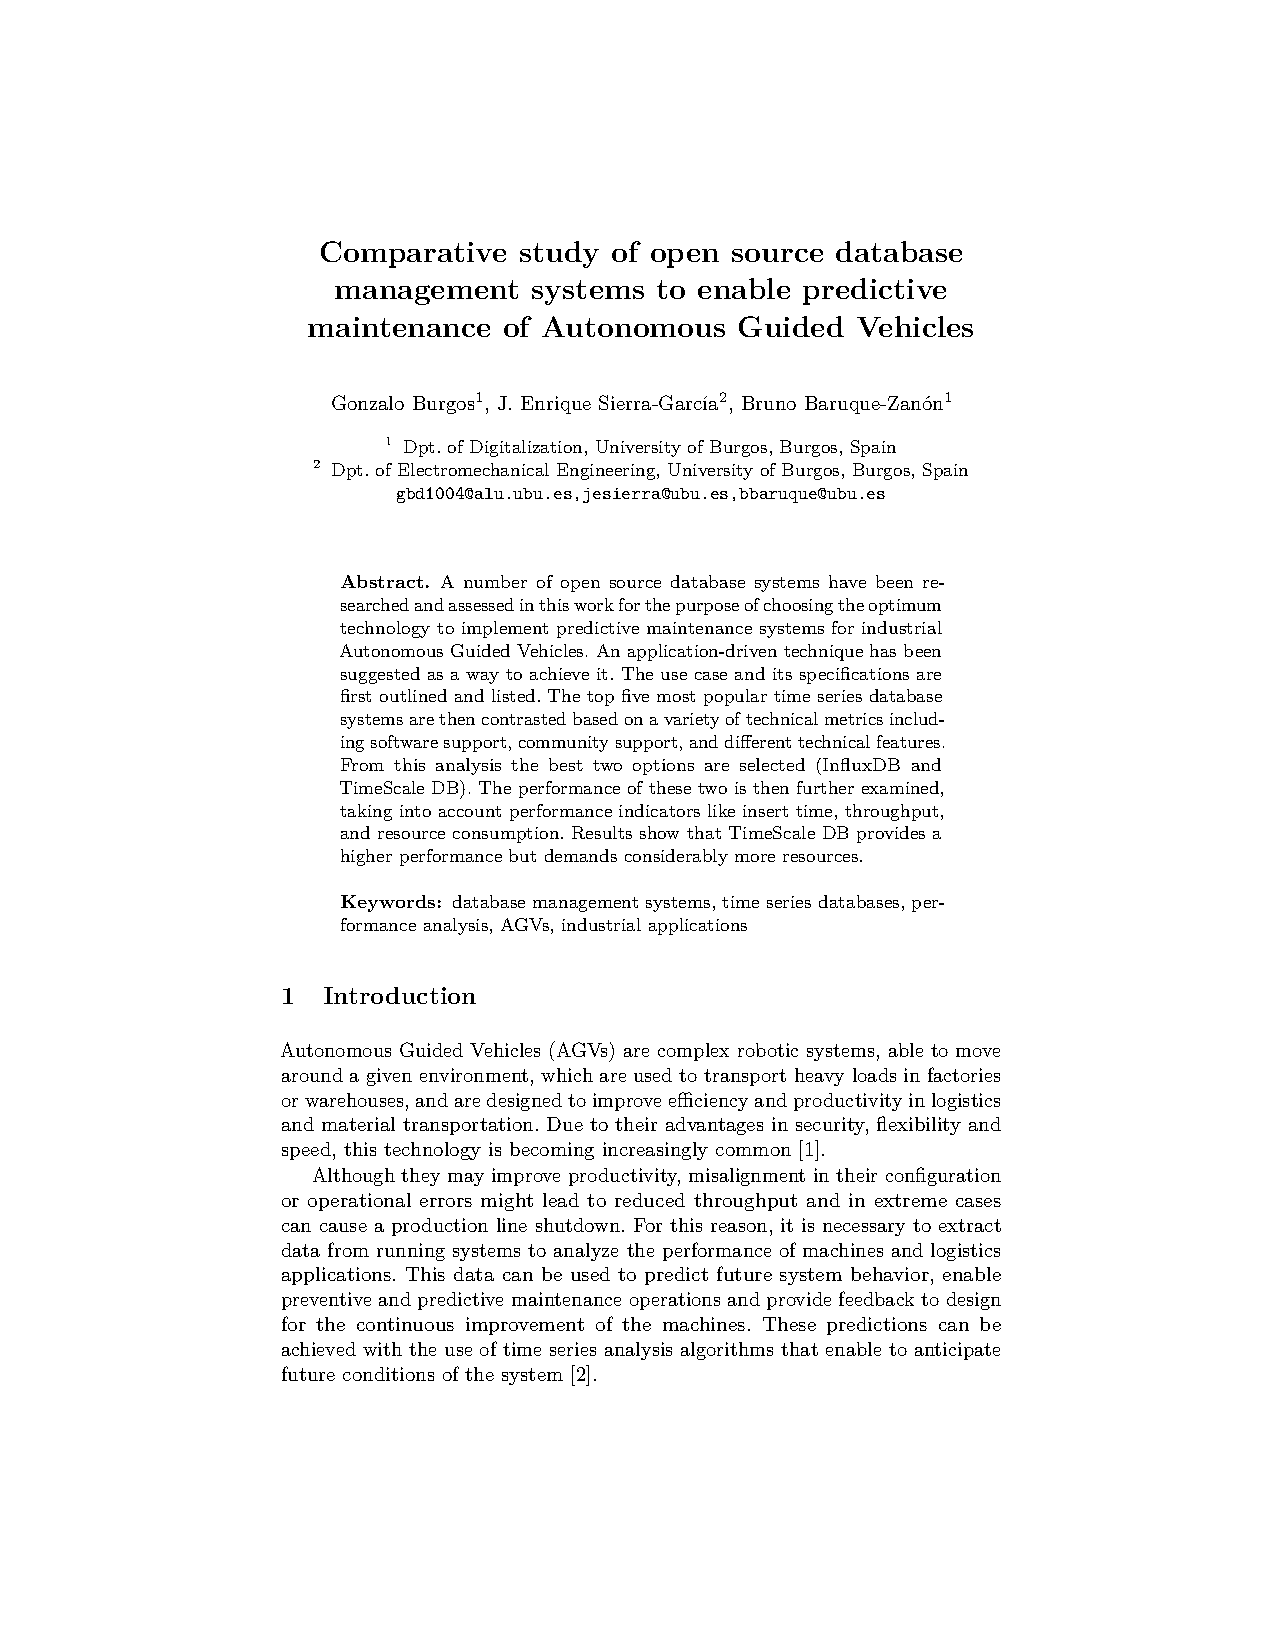
\includepdf[pages=-]{SOCO8364}


\bibliographystyle{IEEEtran}
\bibliography{bibliografiaAnexos}

\end{document}
